% !TEX root = main.tex
\section{재현 가능한 모델 사례 검증}

\subsection{검증 대상과 독립 비교 방법}
앞 절의 일반 논증과 별도로, 객체·감사 기록·집행 식별자의 연
결을 유한한 실행 사례에서 검사하였다. 보조 자료의 Python
3 프로그램 model\_check.py는 입출력 타입, 정수 회계, 유일
소비 기록과 감사 배열을 표현하는 기호 모델이다. 암호문은 평
문의 타입·위치 대응으로 추상화하고, 식별자는 서로 구별되는
기호로 둔다. 암호화·영지식증명·역할 인증·RPC 인증을 구현한
프로그램은 아니다. 정책 선택, 문서 결합과 키 전달의 실제 집
행도 이 검사 범위 밖이다.

검사할 추적 알고리즘은 생성 기록 색인, 감사 평문 슬롯과
타입별 소비 색인을 읽는다. 독립 기대값은 같은 사례의 원래
입력·출력 목록에서 만든 간선 집합에 고정점 도달 계산을 적용
하여 구한다. 이 계산은 감사 슬롯이나 소비 색인을 읽지 않는
다. 두 경로가 반환한 객체·이벤트 정점, 간선과 타입별 미소비
집합을 대조한다. 이는 추적 결과를 그대로 기대값에 복사하는
검사와 구분된다. 유효 관계의 가정 자체나 모든 가능한 이력에
대한 암호 보안을 입증하는 검사는 아니며, 공통 사례 자료의 오
류 가능성도 남는다.

네 사례군은 생산·이전·가공·발급, 분기 후 재합류·종료, 이
전 증표 회수, 질량 0 출력의 탄소 배분이다. 각 사례의 비어 있

% Source PDF page 15, column 2
지 않은 모든 접두 이력에서 존재하는 모든 객체와 이벤트를 시
작점으로 선행·후속 추적을 대조하였다. 총 334개 추적 비교에
서 두 계산의 정점·간선·미소비 집합이 같았다. 이는 선택한 네
그래프 안의 시작점·시점에 대한 결과이며, 모든 그래프나 모든
가능한 상태 변화의 전수 검증은 아니다.

모델과 독립 계산은 record 시작을 통상 event reachability
로 처리하므로 규범의 시작점 규칙 전체와는 다르다. 예를 들
어 Entry \(e→a\)에서 모델의 후속 결과는 \(e,a\)와 출력 간선을 포
함하나 규범은 \(a\)만 포함한다. 선행 record 시작에서는 모델이
\(e\)만 포함하나 규범은 \(e,a\)와 출력 간선을 포함한다. 따라서 334
건은 이 두 모델 계산의 일치이며 추적 보조논증의 규범상 시작
점 처리 전체를 검증한 수치가 아니다. 정리의 증명과 이 제한
된 검사 결과를 구분하고 기존 프로그램·수치를 보존한다.

\subsection{생산·이전 후 사후 대응 사례}
Fig. 1는 입력 \(A\)의 인정 근거가 이력 생성 후 문제로 지정된 가
상 사례다. \(A\)의 \((q,a,e)=(12,6,12)\)를 같은 값 \((6,3,6)\)의
\(B,C\)로 분할한다. \(B\)를 전량 이전하고 운송 탄소 2를 더하면
이전 증표 \(V=(6,3,8)\)과 잔여 회계 증표 \(Z=(0,0,0)\)가 생
긴다. 수신자는 \(V\) 를 같은 회계 값의 \(D\)로 인수한다. 별도 등록
한 \(X=(2,1,2)\)와 \(D\)를 가공하고 공정 탄소 1을 더하여 일반
용 \(E=(7,4,11)\)과 폐기물 \(W=(1,0,0)\)를 만든다. 다른 분
기의 \(C\)는 이미 제품 주장 \(K\)로 발급되었다고 둔다.

이 시점에 \(A\)에서 후속 추적을 하면 \(Z,E,W\) 가 전체 미소비
대상이다. \(X\)는 합류한 이벤트의 다른 부모이므로 후속 추적
이 그 선행 경로를 역으로 확장하지 않는다. \(K\)는 감사 결과의
종단으로 남지만 상태 변경 대상은 아니다. \(Z\)는 질량이 0이고
\(W\) 는 폐기물이지만 종료로 소비할 수 있어 대상에서 제외하지
않는다. 셋을 차단하면 \(E\)의 추가 가공·이전·발급 및 \(Z,W\) 의 종
료도 현재 상태 검사에서 거부된다. 이와 별도로 등록한 정상
객체 \(Y\) 는 차단 대상에 포함되지 않는다.

기준 시점을 \(V\) 의 인수 이전으로 옮기면 대상은 \(C,V,Z\)이다.
그 이후 \(V\) 의 인수가 동결보다 먼저 수락되면, 이전 기준의 실행
은 \(V\) 를 제거하여 완료를 보고하지 않고 소비 경합으로 남긴다.
새 기준의 후속 감사는 \(D\) 이후의 현재 대상을 조사한다. 이 사
례는 사후 대응이 이미 발급된 모든 DPP를 철회한다는 의미가
아니라, 남아 있는 생산·이전 회계 분기의 다음 사용을 제한한
다는 범위를 보여 준다.

\subsection{실패 사례와 검사 결과}
Table 5는 동일 모델에서 실행한 추가 검사를 요약한다. 모든
소비 이벤트 종류에 대해 유효한 사례의 입력 하나를 동결 또는
사용 금지 상태로 바꾸어 해당 소비가 거부되는지 확인했다. 인
수·회수는 같은 이전 증표의 동일 식별자를 사용하며, 어느 경
로를 먼저 수락해도 다른 경로를 같은 상태에서 다시 수락할 수
없었다. 불명확한 제출, 대상 누락, 부분 동결과 소비 경합은 전
체 완료로 판정되지 않았다. 오류를 삽입한 감사 조회는 실패로
끝났으며, 자료가 없다는 응답을 미소비라는 인증된 응답으로
대체하지 않았다.

완료 검사는 소비·상태 전이를 실제로 순서대로 적용하고 각
시점의 상태를 보존하는 별도 이력 모델에서 수행했다. 감사 실
행의 대상과 \(H_{t}\)는 추적을 수행한 스냅샷에 고정하며, 결과의 관
찰 시점과 \(H_{r}\)도 같은 이력에서 얻는다. 예를 들어 \(H_{8}\)의 대상
\(\{E,W,Z\}\)를 차례로 동결하면 \(H_{11}\)에서 완료할 수 있지만, 같

% Source PDF page 16, column 1
은 대상을 존재 이전인 \(H_{1}\)에서 완료했다고 보고할 수는 없다.
다른 실행에서 \(E\)를 동결하고 해제한 뒤 \(W,Z\)를 동결하면 세 성
공 영수증이 있어도 전체가 동시에 차단된 스냅샷이 없었다. 이
실행은 미완료로 남고, \(E\)의 재동결 제출을 실제 수락한 뒤에만
완료로 바뀐다. 상태 변경 로그를 별도로 재생하여 저장된 상태
와도 대조하였다. 이 로컬 시점 연결은 외부 합의·RPC 인증의
구현이나 모든 경합 순서에 대한 전수 검증을 대신하지 않는다.

전체 407개 확인 항목에는 334개 추적 대조, 선택한 실패 사
례와 순차 상태·경합 실행, 소비 상태 검사와 두 인터페이스·회
계 반례가 포함된다. 반례의 “통과”는 취약한 조건이 안전하다
는 뜻이 아니라, 주장한 허용 실행 또는 가정 누락의 결과가 재
현되었다는 뜻이다. 예를 들어 질량 0 출력에 탄소 잔여가 귀속
되는 사례는 XI절의 한계와 동일한 값으로 재현된다.

보조 자료에는 사례 정의, 프로그램, 실행 명령과 원시 JSON
결과를 포함한다. python3 model\_check.py --output
results.json으로 재실행할 수 있다. 실행은 무작위 표본을
사용하지 않으며, 결과에는 소스 해시와 각 확인 항목을 남긴다.
이 결과는 구체 암호 방식, 실제 회로·계약·클라이언트의 적합
성, 성능이나 외부 자료의 진실성을 입증하지 않는다. 또한 같
은 의무를 구현한 조합 기준선 \(C^{\star }\)가 같은 검사를 통과하는 것
과 양립한다.

% Source PDF page 16, column 2


\begin{table}[htbp]\centering\small
    \setcounter{table}{4}\caption{Symbolic checks and their observed outcomes}
    \begin{tabularx}{\linewidth}{@{}XX@{}}\toprule
        \textbf{Case}                        & \textbf{Outcome in the finite model}                  \\ \midrule
        All fixture starts and prefixes      & 334 exact graph/frontier matches                      \\
        Join, backward sibling, other parent & Reachable edges retained; unrelated branches excluded \\
        Voucher resolution order             & First consumption excludes the competing path         \\
        Frozen/revoked input                 & All eight consuming event kinds rejected              \\
        Missing/mistyped audit data          & Trace failure                                         \\
        Partial, omitted or pending result   & Incomplete response                                   \\
        Race or incompatible checkpoint      & Incomplete response                                   \\
        Zero-mass carbon residual            & Permitted accounting counterexample                   \\
        Owner-secret alias                   & Identifier-invariance countermodel                    \\
        \bottomrule\end{tabularx}\end{table}
\begin{figure}[htbp]\centering
    \includegraphics[page=16,trim=46 687 44 47,clip,width=\linewidth]{source.pdf}
    \caption{Worked accounting flow after accepted production and transfer. The dashed edge is an actual input edge outside the forward traversal from A; the figure shows it only to explain the process accounting.}
\end{figure}
